%! TEX root = ../main.tex
\documentclass[main]{subfiles}

\begin{document}
\silentchapter{\texorpdfstring
{$e^x, \sin x(\cos x), x^\alpha, \log x$  の積$\rightarrow$部分積分}
{}}

\begin{mondai}{8}{今週の積分}{**}
    \begin{align*}
        \int_1^e \sqrt{x}\log x dx
    \end{align*}
\end{mondai}

\approachitem{$e^x, \sin x(\cos x), x^\alpha, \log x$  の積$\rightarrow$部分積分}

\solutionhead
\hfill
以下に計算手順を示す.
\hfill\

\begin{align*}
    \int_1^e \sqrt{x}\log x dx
        &= \left[\frac{2}{3}x^\frac{3}{2}\log x\right]_1^e-\int_1^e \frac{2}{3}x^\frac{3}{2}\cdot x^{-1}dx \\
        &= \frac{2}{3}e^\frac{3}{2}-\frac{2}{3}\int_1^ex^\frac{1}{2} dx \\
        &= \frac{2}{3}e^\frac{3}{2}-\frac{2}{3}\left[\frac{2}{3}x^\frac{3}{2}\right]_1^e \\
        &= \frac{2}{3}e^\frac{3}{2}-\frac{4}{9}\left(e^\frac{3}{2}-1\right) \\
        &= \boldsymbol{\frac{2}{9}e\sqrt{e}+\frac{4}{9}}
\end{align*}

\begin{figure}[H]
    \centering
    % 座標系のスケールを調整して見やすくする
    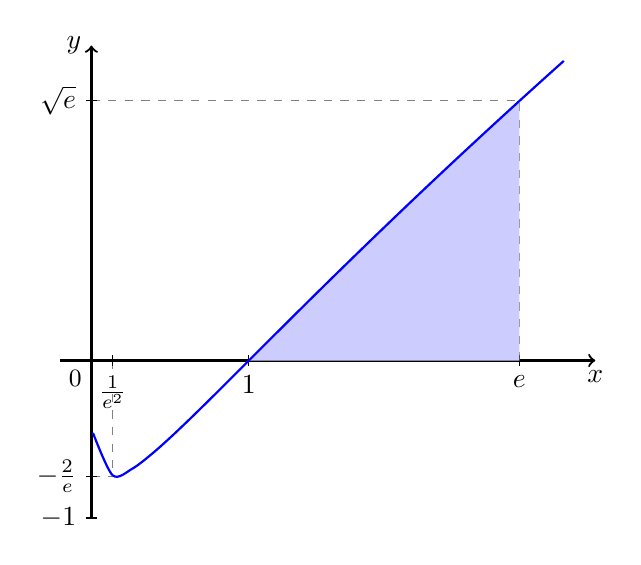
\begin{tikzpicture}[x=2cm, y=2cm]
        % --- 座標軸の描画 ---
        \draw[->, thick] (-0.2,0) -- (3.2,0) node[below] {$x$};
        \draw[->, thick] (0,-1) -- (0,2) node[left] {$y$};

        % --- グリッド線の描画 ---
        \draw[gray, thin, dashed] (2.718,0) -- (2.718,1.65);
        \draw[gray, thin, dashed] (0,1.65) -- (2.718,1.65);
        \draw[gray, thin, dashed] (0,-0.736) -- (0.135,-0.736);
        \draw[gray, thin, dashed] (0.135,0) -- (0.135,-0.736);

        % --- 目盛りの描画 ---
        % x軸の目盛りとラベル
        \foreach \x/\label in {0.135/\frac{1}{e^2}, 1/1, 2.718/e} {
            \draw (\x, 2pt) -- (\x, -2pt) node[below] {$\label$};
        }
        \node[below left, font=\small] at (0,0) {$0$};

        % y軸の目盛りとラベル
        \draw (2pt, -1) -- (-2pt, -1) node[left] {$-1$};
        \draw (2pt, 1.65) -- (-2pt, 1.65) node[left] {$\sqrt{e}$};
        \draw (2pt, -0.736) -- (-2pt, -0.736) node[left] {$-\frac{2}{e}$};

        % ★★★ 1. 1からeの範囲で領域を塗りつぶす ★★★
        % グラフの線を描く前に塗りつぶしを行う
        \fill[blue!20] (1,0) -- plot[domain=1:2.718, smooth, variable=\x] ({\x}, {sqrt(\x)*ln(\x)}) -- (2.718,0) -- cycle;

        % --- 関数のプロット ---
        % 【注意】log(0)は定義されないため、0より少し大きい値から開始
        \draw[
            domain=0.01:3,
            smooth,
            variable=\x,
            blue,
            thick
        ] plot ({\x}, {sqrt(\x)*ln(\x)}); % logは自然対数 ln() で計算

    \end{tikzpicture}
    \caption{$y=\sqrt{x}\log x$ のグラフと $1 \le x \le e$ の領域}
    \label{fig:sqrt_log_filled_tikz}
\end{figure}

\end{document}